\documentclass[a4paper, 12pt]{article}
\usepackage{cmap}
\usepackage{amssymb}
\usepackage{amsmath}
\usepackage{graphicx}
\usepackage{floatflt}
\usepackage{amsthm}
\usepackage{upgreek}
\usepackage{setspace}
\usepackage[T2A]{fontenc}
\usepackage[utf8]{inputenc}
\usepackage[normalem]{ulem}
\usepackage{mathtext} % русские буквы в формулах
\usepackage[left=2cm,right=2cm, top=2cm,bottom=2cm,bindingoffset=0cm]{geometry}
\usepackage[english,russian]{babel}
\usepackage[unicode]{hyperref}
\newenvironment{Proof} % имя окружения
{\par\noindent{$\blacklozenge$}} % команды для \begin
{\hfill$\scriptstyle\boxtimes$}
\newenvironment{example} % имя окружения для примеров
{\par\noindent{\textsc{\textbf{Пример}.}}} % символ рядом с \begin
{\hfill$\scriptstyle\Box$} % символ рядом с \end
\newcommand{\Rm}{\mathbb{R}}
\newcommand{\Cm}{\mathbb{C}}
\newcommand{\Z}{\mathbb{Z}}
\newcommand{\I}{\mathbb{I}}
\newcommand{\N}{\mathbb{N}}
\newcommand{\p}{\prime}
\newcommand{\Ra}{\Rightarrow}
\newcommand{\ra}{\rightarrow}
\newcommand{\FI}{\Phi}
\newcommand{\Sp}{\text{Sp}}
\renewcommand{\leq}{\leqslant}
\renewcommand{\geq}{\geqslant}
\renewcommand{\alpha}{\upalpha}
\renewcommand{\beta}{\upbeta}
\renewcommand{\gamma}{\upgamma}
\renewcommand{\delta}{\updelta}
\renewcommand{\d}{\partial}
\renewcommand{\Re}{\operatorname{Re}}
\renewcommand{\Im}{\operatorname{Im}}
\newcommand{\Ln}{\operatorname{Ln}}
\newcommand{\Arccos}{\operatorname{Arccos}}
\newcommand{\Arcsin}{\operatorname{Arcsin}}
\renewcommand{\varphi}{\upvarphi}
\renewcommand{\tau}{\uptau}
\renewcommand{\rho}{\uprho}
\renewcommand{\lambda}{\uplambda}
\renewcommand{\psi}{\uppsi}
\renewcommand{\xi}{\upxi}
\renewcommand{\epsilon}{\upvarepsilon}
\newcommand{\limdef}{\forall \epsilon >0\ \exists \delta (\epsilon) > 0}
\newcommand\Norm[1]{\left\| #1 \right\|}
\newcommand\ef[1]{e^{i#1}}
\newcommand{\Arg}{\operatorname{Arg}}
\newtheorem*{theorem}{Теорема}
\newtheorem*{cor}{Следствие}
\newtheorem*{lem}{Лемма}
\title{\vspace{6.5cm}\textbf{\Huge{Теория функции комплексного переменного}}\\Конспект по 2 курсу 
	специальности «прикладная математика»\\(лектор А. А. Леваков)}
\date{}
\begin{document}
	\maketitle
		\newpage
	\tableofcontents{}
	\newpage
	\section{Комплексные числа.}
	$\bullet$ \textit{Под \textbf{множеством комплесных чисел} $\Cm$ понимают множество упорядоченных пар $(a,b)$ вещественных чисел таких, что на этом множестве введены 3 операции}\begin{enumerate}
		\item $(a_1,b_1) = (a_2,b_2) \Longleftrightarrow a_1 = a_2, b_1 = b_2$;
		\item $(a_1,b_1) + (a_2, b_2) = (a_1+a_2, b_1 + b_2)$;
		\item $(a_1, b_1)\cdot (a_2,b_2) = (a_1a_2 - b_1b_2, a_1b_2 + a_2b_1)$;
	\end{enumerate}
Комплексное число обычно обозначается символом $z$.\\\\
\noindent
\parbox[b][3.5cm][t]{10mm}{
	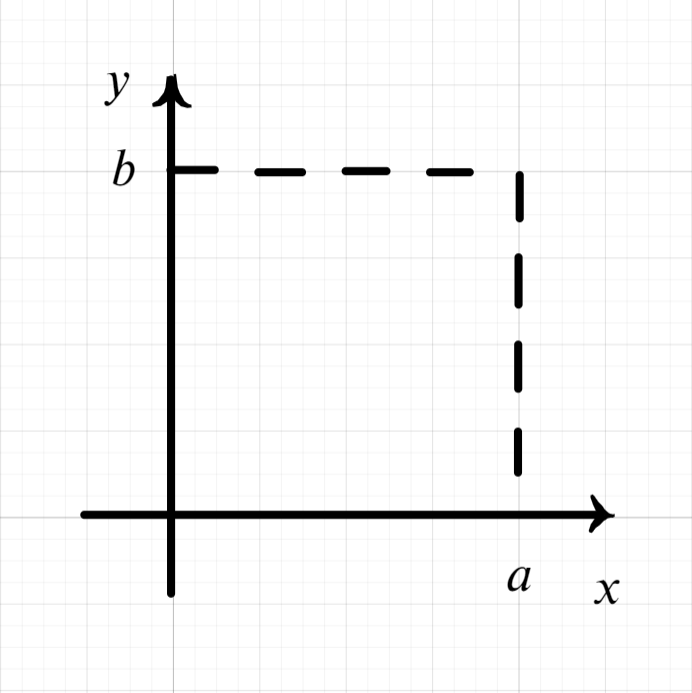
\includegraphics[scale=0.25]{images/001.png}}
\hfill
\parbox[b][2.75cm][t]{115mm}{
Между множеством комплесных чисел и множеством точек ДПСК существует взаимнооднозначное соответствие.\\\\
$\bullet$ \textit{Плоскость с выбранной на ней ДПСК, на которой изображаются комплексные числа, называется \textbf{комплексной плоскостью}.}}\\\\
\noindent
\parbox[b][4cm][t]{110mm}{
Также существует взаимнооднозначное соответствие между множеством комплексных чисел и множеством векторов.\\\\
$\bullet$\textit{ Точки, соответствующие комплексным числам $(a,0)$ лежат на оси $x$. Тогда $(a,0) = a$, а ось $x$ называется \textbf{вещественной}.}}
\hfill
\parbox[b][5cm][t]{55mm}{
	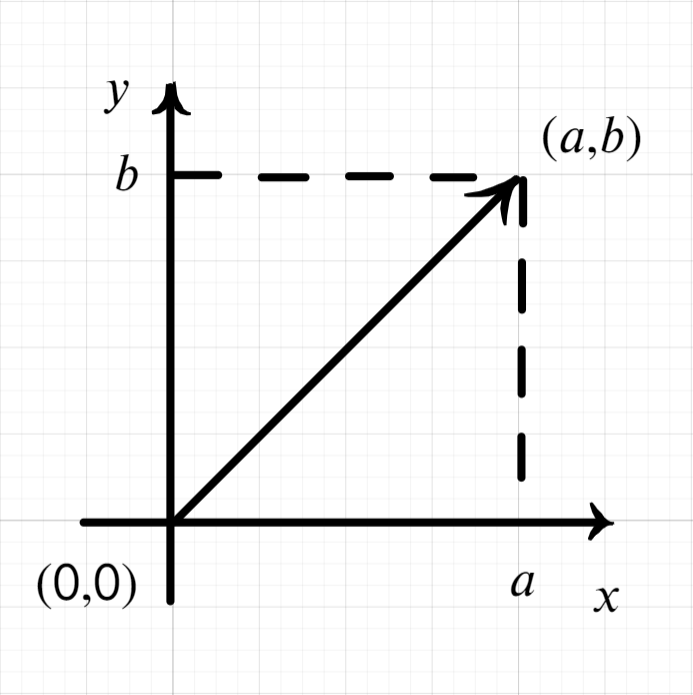
\includegraphics[scale=0.25]{images/002.png}}\\
На множестве комплексных чисел $(0,1)\cdot (0,1) = (-1,0) = -1.$ То есть среди комплексных чисел есть такое число $(0,1) = i$, что $i^2 = 1$.\\\\
$\bullet$ \textit{Точки, соответствующие комплексным числам $(0,b)$ лежат на оси $y$. Тогда $(0,b) = bi$, а ось $y$ называется \textbf{мнимой}}.\\\\
Возьмем произвольное комплексное число $(a,b)$.
$$(a,b) = (a,0) + (b,0) = a+ (b,0)\cdot (0,1) = a+bi.$$
Следовательно, любое комплексное число можно записать в виде $z = a+bi$.\\\\
$\bullet$ \textit{Такая форма записи комплексного числа называется \textbf{алгебраической формой записи}.}\\\\
Как правило, будем записывать комплексные числа в алгебраической форме.\\\\
$\bullet$ \textit{Число $\sqrt{a^2 + b^2} = |z|$ называется \textbf{модулем} комплексного числа.}\\\\
Геометрически это расстояние от начала координат до точки, соответствующей комплексному числу.\\
\noindent
\parbox[b][4.5cm][t]{95mm}{
	$\bullet$ \textit{Угол, который образует вектор к числу $z$ с осью $x$ называется \textbf{аргументом} комплексного числа и обозначается $\varphi = \arg (z)$.}\\\\
	Причем, если вращение вектора от оси $x$ против часовой стрелки, то аргумент считаем положительным. Иначе отрицательным.
	}
\hfill
\parbox[b][5cm][t]{70mm}{
	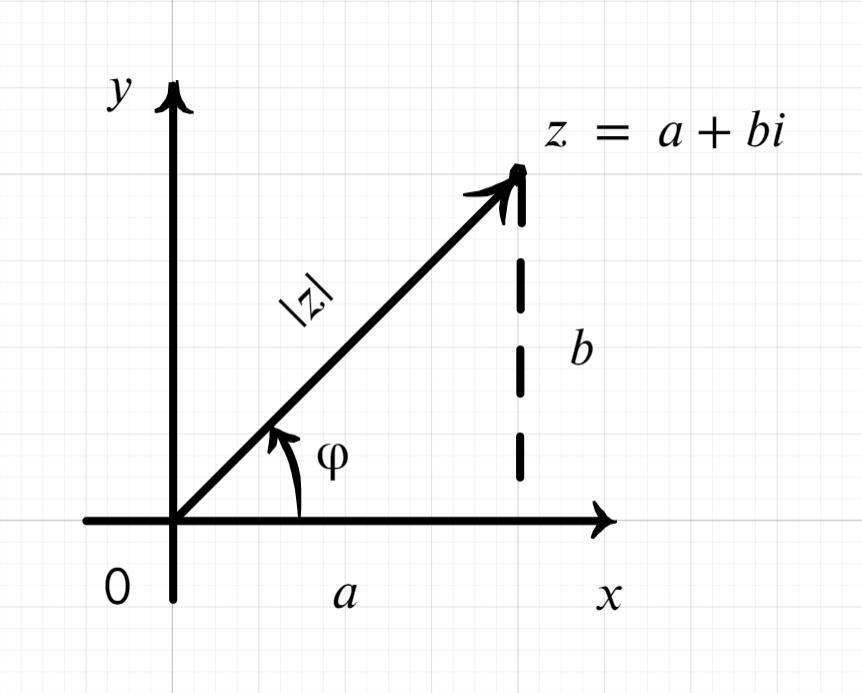
\includegraphics[scale=0.25]{images/003.png}}\\
 Если $\varphi$ --- аргумент, то чиcла $\varphi + 2\pi k$, $k\in \Z$ также являются аргументами (то есть аргумент определен неоднозначно). Обозначаем \begin{itemize}
	\item $\Arg(z) = \varphi + 2\pi k$ --- все значения аргумента;
	\item $\arg (z) = \varphi$ --- одно значение аргумента.
\end{itemize}
Чаще всего $\varphi \in (-\pi; \pi]$. Но иногда удобно считать, что $\varphi \in [0;2\pi)$.\\\\
$\bullet$ \textit{Это фиксированное значение аргумента называется \textbf{главным значением аргумента} комплексного числа.}\\\\
Таким образом, $a = |z|\cos \varphi$, $b = |z|\sin\varphi$. Тогда можно записать $$z = a + bi = |z|\cdot (\cos \varphi + i\sin\varphi).$$
$\bullet$ \textit{Такая форма записи комплексного числа называется \textbf{тригонометрической формой записи}}.\\\\
Введем функцию $e^{i\varphi}$ опеределенную на множестве $\Rm$ и принимающую значения в множестве $\Cm$ по формуле $$e^{i\varphi} = \cos\varphi + i\sin\varphi.$$
Используя эту функцию, можем записать комплексное число в виде $$z = a+bi = |z|\cdot e^{i\varphi}.$$
$\bullet$ \textit{Такая форма записи комплексного числа называется \textbf{экспоненциальной формой записи}}.\\\\
Покажем, что функция $e^{i\varphi}$ обладает свойствами экспоненты:
\begin{enumerate}
	\item $\ef{\varphi_1}\cdot \ef{\varphi_2} = \ef{(\varphi_1 + \varphi_2)}$.
	\begin{Proof}
		\begin{multline*}
			\ef{\varphi_1}\cdot \ef{\varphi_2} = (\cos\varphi_1, \sin\varphi_1)\cdot (\cos\varphi_2, \sin\varphi_2) =\\= (\cos\varphi_1\cos\varphi_2-\sin\varphi_1\sin\varphi_2,\ \cos\varphi_1\sin\varphi_2 + \sin\varphi_1\cos\varphi_2)=\\=(\cos(\varphi_1 + \varphi_2),\ \sin(\varphi_1 + \varphi_2)) = \ef{\varphi_1 + \varphi_2}.
		\end{multline*}
	\end{Proof}
\item $\dfrac{\ef{\varphi_1}}{\ef{\varphi_2}} = \ef{(\varphi_1 - \varphi_2)}.$
\item $(\ef{\varphi})^n = \ef{n\varphi}$, $n\in \N$.
\end{enumerate}
\noindent
\parbox[b][4cm][t]{90mm}{
	Возьмем комплексную плоскость и обозначим на ней 2 комплексных числа и соответствующие им радиус-векторы. Построим параллелограмм на этих векторах и возьмем его диагональ. Комплексное число, соответствующее этой диагонали, имеет вид $z_3 = (a_1 + a_2, b_1 + b_2)$, то есть является суммой комплексных чисел $z_1$ и $z_2$.
	}
\hfill
\parbox[b][5cm][t]{70mm}{
	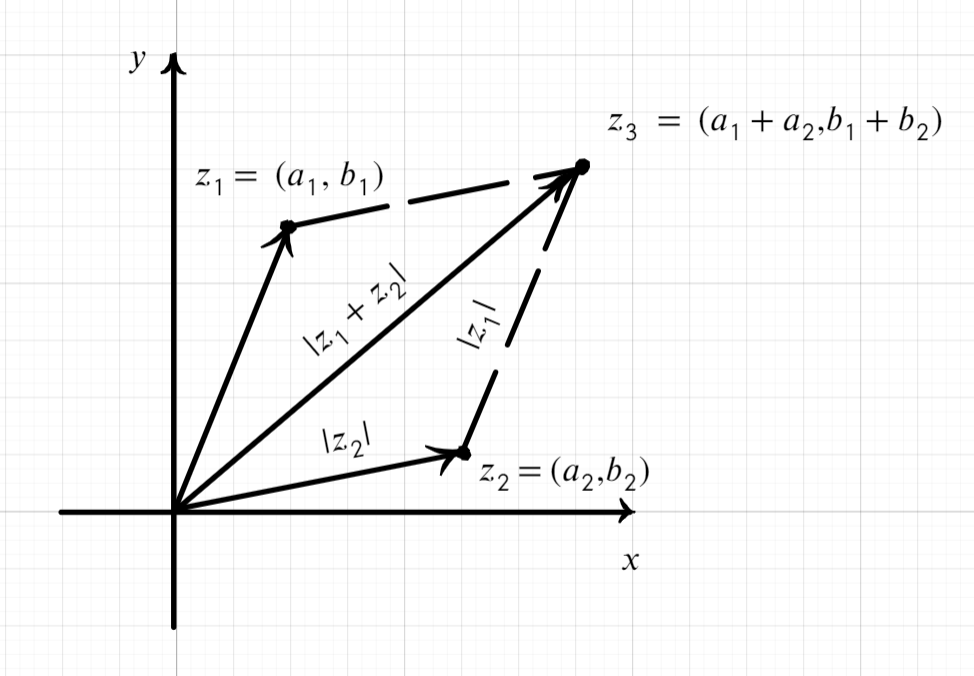
\includegraphics[scale=0.3]{images/004.png}}\\\\
Разность комплексных чисел $z_1-z_2 = z_1 + (-z_2)$ определяется вектором, который является второй диагональю параллеограмма построенного на векторах $z_1$ и $z_2$.
$$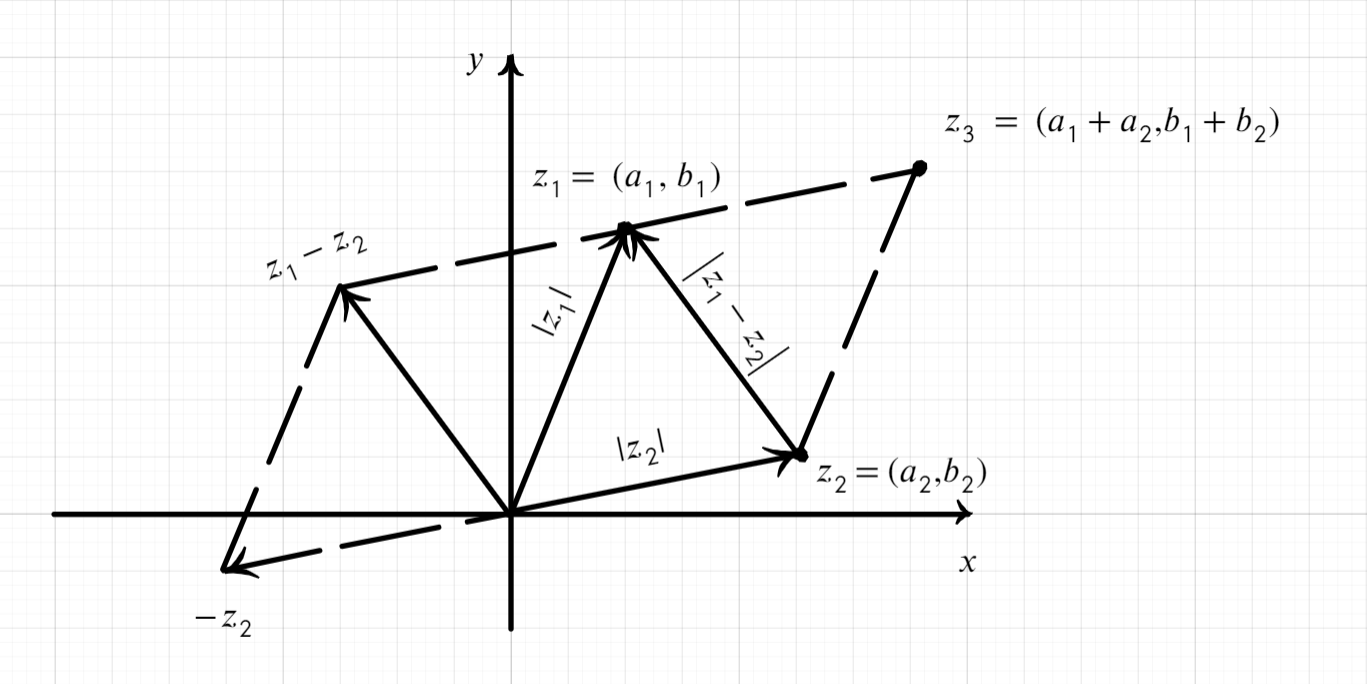
\includegraphics[scale=0.4]{images/005.png}$$
Из графиков следует свойство
$$\big||z_1|-|z_2|\big|\leqslant |z_1 + z_2|\leqslant |z_1| + |z_2|.$$
Из свойств комплексных чисел\\\\
$z_1\cdot z_2 = |z_1|\cdot \ef{\varphi_1}\cdot |z_2|\cdot \ef{\varphi_2} = |z_1|\cdot |z_2| \cdot \ef{(\varphi_1 + \varphi_2)}.$\\\\
$\dfrac{z_1}{z_2} = \dfrac{|z_1|\cdot \ef{\varphi_1}}{|z_2|\cdot \ef{\varphi_2}} = \dfrac{|z_1|}{|z_2|}\cdot \ef{(\varphi_1 - \varphi_2)}.$\\\\
Отсюда вытекает, что
\begin{enumerate}
	\item $|z_1\cdot z_2| = |z_1|\cdot |z_2|$,\quad $\arg(z_1\cdot z_2) = \arg (z_1) + \arg (z_2)$.
	\item $\Big|\dfrac{z_1}{z_2}\Big|=\dfrac{|z_1|}{|z_2|}$, \quad $\arg\Big(\dfrac{z_1}{z_2}\Big) = \arg(z_1) - \arg(z_2)$.
 \end{enumerate}
$\bullet$ \textit{Если число $z = a+bi$ --- комплексное число, то число $\overline{z} = a - bi$ называется \textbf{сопряженным} к комплексному числу $z$.}\\\\
Тогда $z\cdot \overline{z} = a^2 + b^2 = |z|^2.$ Из свойств множества комплексных чисел $$z_1=z_2 \Longleftrightarrow a_1 = a_2,\ b_1 = b_2.$$
В экспоненциальной форме
$$|z_1|\cdot\ef{\varphi_1} = |z_2|\cdot\ef{\varphi_2}\Longleftrightarrow |z_1| = |z_2|,\ \arg(z_1) = \arg(z_2) + 2\pi k,\ k\in \Z.$$
$\bullet$ \textit{\textbf{Корнем n-ой степени} комплексного числа $z$ называется такое число $\upzeta$, что $\upzeta ^ n = z$. Обозначение: $\sqrt[n]{z}$.}\\\\
Пусть $z = |z|\cdot \ef{\varphi}$, $\upzeta = |\upzeta|\cdot \ef{\varphi_1}$. Тогда $$(|\upzeta|\cdot \ef{\varphi_1})^n = |z|\cdot  \ef{\varphi}.$$
$$|\upzeta|^n\cdot\ef{n\varphi_1} = |z|\cdot \ef{\varphi}.$$
Тогда получаем
	\begin{align*}
		|\upzeta|^n = |z| &\Rightarrow |\upzeta| = |z|^{\frac1n}.\\
		n\varphi_1 = \varphi + 2\pi k,\ k \in \Z &\Rightarrow \varphi_1 = \dfrac{\varphi + 2\pi k}{n}.
	\end{align*}
Значит $$\upzeta = |z|^{\frac{1}{n}}\cdot \ef{\frac{\varphi + 2\pi k}{n}}.$$
\noindent
\parbox[b][8.5cm][t]{10mm}{
	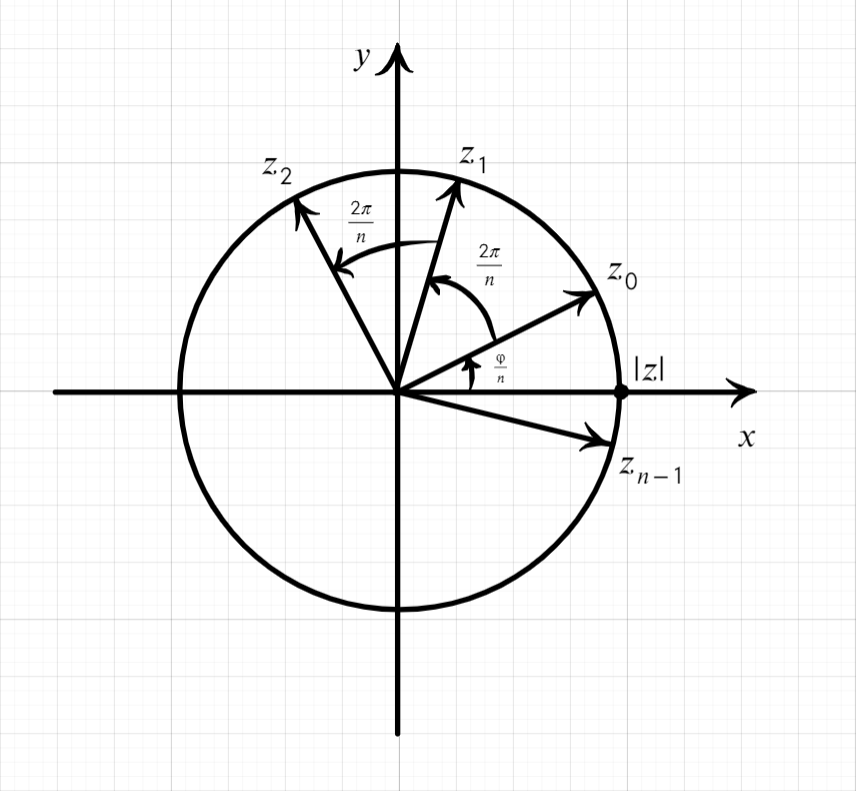
\includegraphics[scale=0.4]{images/006.png}}
\hfill
\parbox[b][6.5cm][t]{65mm}{
	При $k = 0$ получаем $z_0$,\\\\ $k=1\to z_1$,\\\\ $k=2\to z_2$,\\\ $\ldots$,\\\\ $k=n-1\to z_{n-1}$,\\\\ $k = n\to z_0$. }\\
Следовательно, корень $n$-ой степени из любого ненулевого комплексного числа имеет ровно $n$ различных значений. То есть $\sqrt[n]{z} = \upzeta_k$ и $$\upzeta_k = |z|^{\frac1n}\cdot \ef{\frac{(\arg z + 2\pi k)}{n}},\quad k = 0,1,\ldots,n-1.$$
\section{Комплексные функции.}
Пусть $D\subseteq \Rm$, $f:D\to\Cm$.\\\\
$\bullet$ \textit{Функция $w=f(t)$, $t\in D\in\Rm$ называется \textbf{комплекснозначной} функцией.}\\\\
Запишем в алгебраической форме:
$$w=u(t)+i\cdot v(t),\quad \Re (w) = u(t)\in\Rm,\ \Im (w) = v(t)\in\Rm.$$
Производная и интеграл для таких функций определяются аналогично вещественным функциям:
$$w(t)^\p = u^\p + i\cdot v^\p.$$
$$\int\limits_{a}^bw(t)dt = \int\limits_{a}^bu(t)dt + i\cdot \int\limits_{a}^bv(t)dt.$$
Рассмотрим функцию $w = e^{it}$, $t\in[0;2\pi)$. Ее можно представить как $e^{it} = \cos t + i\cdot \sin t.$ Тогда производная от этой функции равна $$(e^{it})^\p = -\sin t + i\cdot \cos t = i\cdot (\cos t + i\cdot \sin t) = ie^{it}.$$
Пусть $f : D\to \Cm$, $D\in \Cm$.\\\\
$\bullet$\textit{ Функция $w = f(z)$, $z\in D\in\Cm$ называется \textbf{комплексной функцией}.}\\\\
Это же определение можно сформулировать иначе.\\\\
$\bullet$ \textit{Пусть заданы множества $D\in \Cm$ и $L\in\Cm$ и правило $D\overset{f}{\to}L$, которое каждому значению $z\in D$ ставит в соответствие одно или несколько значений $w \in L$. Это мы и будем понимать под \textbf{комплексной функцией}.}.\\\\
Функцию, ставящую в соответствие одно значение, будем называть \textbf{однозначной}. Аналогично, если два значения, то \textbf{двузначной}. Если неизвестно сколько значений, то \textbf{многозначной}.\\\\
Например, графически двузначная функция будет изображаться таким образом
$$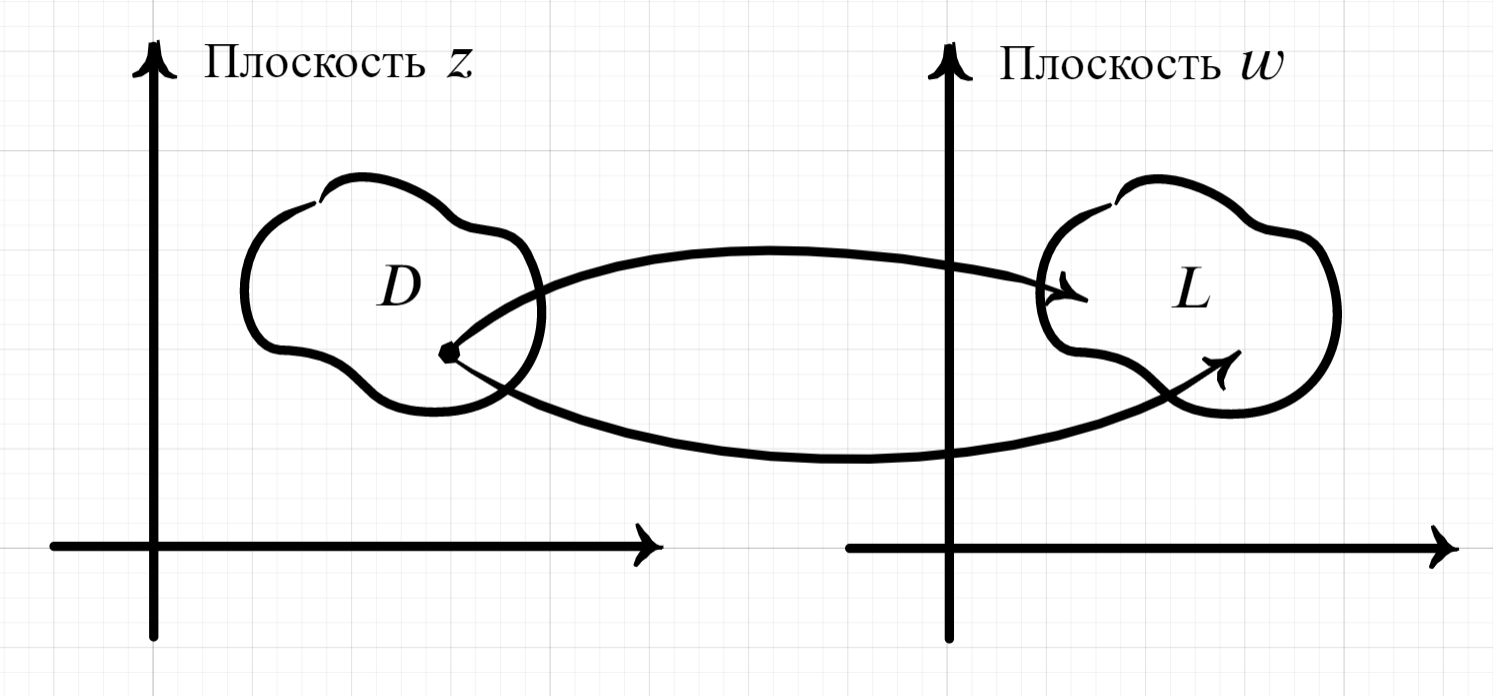
\includegraphics[scale=0.3]{images/007.png}$$
Рассмотрим примеры комлексных функций:\begin{enumerate}
	\item $w = az + b$, $a,b\in \Cm$ --- \textit{\textbf{линейная функция}};
	\item $w = az^2 + bz + c$, $a,b,c\in\Cm$ --- \textbf{\textit{квадратичная функция}};
	\item $w = a_nz^n + a_{n-1}z^{n-1} + \ldots + a_1z + a_0$, $\forall a_i \in \Cm, n\in \N$ --- \textbf{\textit{полином n-ой степени}};\\\\
	Каждый полином $n$-ой степени имеет ровно $n$ корней с учетом кратности.
	\item $w = \sqrt{z}$;\\\\
	Решением этой функции является множество таких $\zeta ^2 = z$, где $$\zeta = |z|^\frac12\ef{\frac{\arg z + 2\pi k}{2}},\quad k = 0,1.$$
	Тогда $\zeta_1 = |z|^\frac12\ef{\frac{\arg z}{2}}$, $\zeta_2 = -|z|^\frac12\ef{\frac{\arg z}{2}}$. Следовательно, $w = \sqrt{z}$ --- двузначная функция.\\\\
	Графически это можно изобразить как $$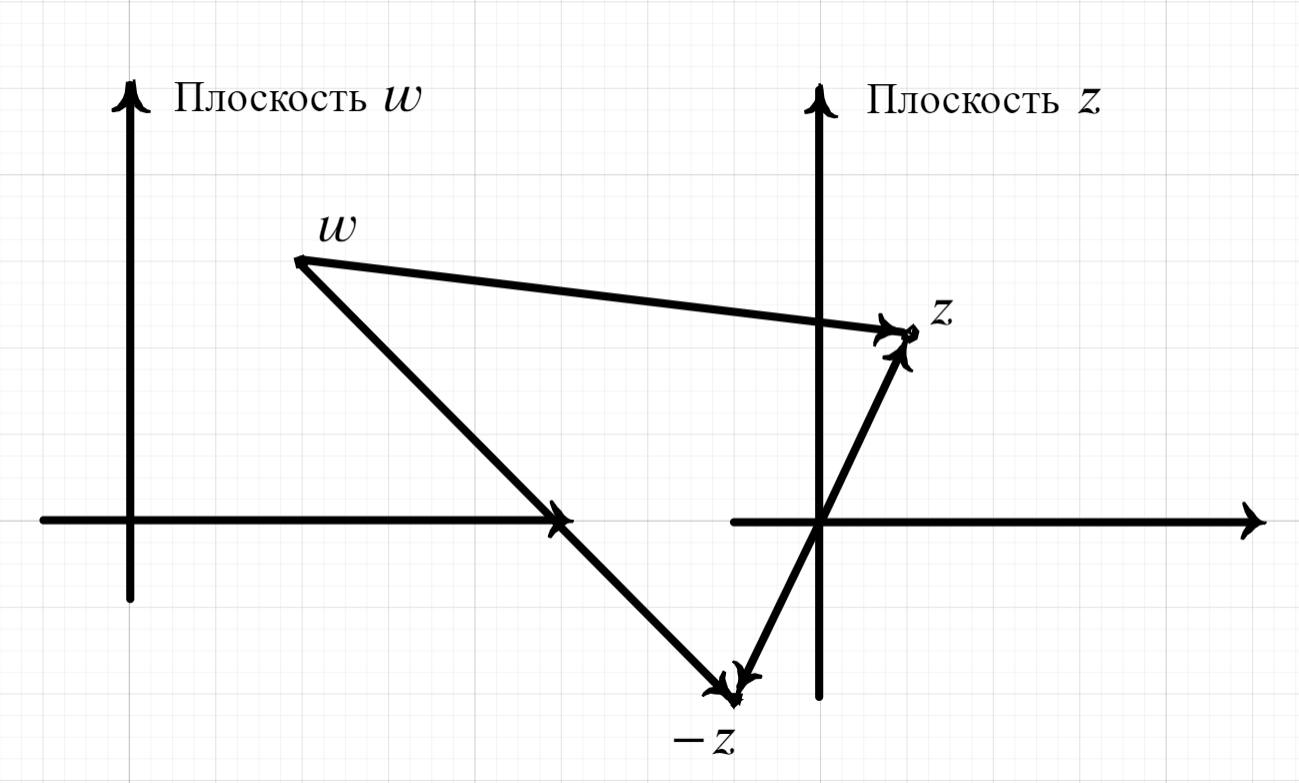
\includegraphics[scale=0.3]{images/008.png}$$
	Функции $w_1 = |z|^\frac12\ef{\frac{\arg z}{2}}$, $w_2 = -|z|^\frac12\ef{\frac{\arg z}{2}}$ являются однозначными. Их также называют \textbf{ветвями} двузначной функции $w = \sqrt{z}$.
	\item $w = e^z$ --- \textbf{\textit{комплексная экспонента}};
	$$e^z = e^{x + iy} = e^x(\cos y + i\cdot \sin y) = e^x\cos y + i\cdot e^x \sin y,$$
	то есть $\Re (e^z) = e^x\cos y$, $\Im(e^x) = e^x\sin y$. Если $z = x$, $e^z = e^x$.\\\\
	Рассмотрим уравнение $w_0 = e^z$, $w_0 \ne 0$. 
	\begin{center}
		$\begin{matrix}
			w_0 = |w_0|\cdot e^{i\arg w_0},\\
			e^z = e^x\cdot e^{iy} = e^x \cdot \ef{\arg z};
		\end{matrix}\quad \Longrightarrow\quad  \begin{matrix}
		|w_0|=e^x,\\
		y = \arg z + 2\pi k,\ k\in \Z.
	\end{matrix}$
	\end{center}
Отсюда $x = \ln|w_0|$, $y = \arg z + 2\pi k$, $k\in\Z$. Тогда множество решений уравнения $w_0 = e^z$ имеет вид $$z = \ln |w_0|+i\cdot (\arg z +2\pi k).$$
\item $w = \Ln z = \ln|z| + i\cdot (\arg z + 2\pi k)$, $k\in \Z$ --- \textbf{\textit{комплексный логарифм}};\\\\
Если $z = x > 0$, то при $k = 0$ получим $\ln z = \ln |z| + i\arg z$ --- главное значение (ветвь) $\Ln z$. Эта функция совпадает с вещественной $\ln x$.\\\\
Из двух предудыщих рассмотренных функций вытекает, что во множестве комплексных чисел уравнение $e^z = -1$ имеет множество решений $\Ln(-1) = i\cdot (\pi+ 2\pi k)$, $k\in \Z$.
\item $w = z^\alpha$, $\alpha \in \Cm$ --- \textbf{\textit{степенная функция с любым показателем}};\\\\
Причем $z ^\alpha = e^{\alpha \Ln z}$ при $z \ne 0$.
\item $w = \sin z$, $w = \cos z$ --- \textbf{\textit{комплексные синунс и косинус}} соответственно;
$$\sin z = \dfrac{e^{iz} - e^{-iz}}{2i},\quad \cos z = \dfrac{e^{iz} + e^{-iz}}{2}.$$
Проверим, что при $z = x$ получим $\sin z = \sin x$:
$$\sin z = \dfrac{e^{ix} - e^{-ix}}{2i}=\dfrac{\cos x + i\sin x - \cos x + i\sin x}{2i} = \sin x.$$
Комплексные синус и косинус являются $2\pi$-периодическими функциями.\\\\
Все формулы для вещественных синуса и косинуса выполняются и для комплексных. Например, $$\cos^2 z + \sin^2z = \Big(\dfrac{e^{iz} + e^{-iz}}{2}\Big)^2 + \Big(\dfrac{e^{iz} - e^{-iz}}{2i}\Big)^2 = \dfrac{e^{2iz} + e^{-2iz} + 2}{4} + \dfrac{e^{2iz} + e^{-2iz} -2}{-4} = 1.$$
Аналогично доказываются 
\begin{center}
	$\cos ^2z -\sin^2z = \cos 2z,\quad 2\sin z\cos z = \sin2z,\quad \sin(z_1 + z_2) = \sin z_1 \cos z_2 + \sin z_2 \cos z_1$ и так далее.
\end{center}
\end{enumerate}
\begin{example}
	Найдем, чему равно $z$ в уравнении $\cos z = A$.\\\\
	$$\cos z = \dfrac{e^{iz} + e^{-iz}}{2} = [e^{iz} = t] = \dfrac{t + \frac{1}{t}}{2} = A\quad\Rightarrow\quad t^2 - 2At + 1 = 0.$$
	Отсюда $$t = \dfrac{2A + \sqrt{4A^2 -4}}{2} = A + \sqrt{A^2 - 1}.$$
	Тогда $$e^{iz} = A + \sqrt{A^2 - 1}.$$
	Следовательно, $$iz = \Ln (A + \sqrt{A^2 - 1})\quad \Rightarrow\quad z = -i\Ln(A + \sqrt{A^2 - 1}).$$
\end{example}\\
Функция \begin{center}
	$w = -i\cdot\Ln(z + \sqrt{z^2 - 1}) = \Arccos z$ --- \textbf{комплексный арккосинус}.
\end{center} Аналогично можно вывести функцию \begin{center}
	$w = -i\cdot\Ln(iz + \sqrt{1 - z^2}) = \Arcsin z$ --- \textbf{комплексный арксинус}.
\end{center}
\section{Предел функции комплексного переменного. Непрерывные функции комплексного переменного.}
$\bullet$ \textit{Последовательность $(z_n)$, где все члены $z_n \in \Cm$ называется \textbf{комплексной последовательностью}.}\\\\
$\bullet$ \textit{Число $a\in \Cm$ называется \textbf{пределом последовательности $(z_n)$}, если} $$\limdef : \forall n \geqslant \delta (\epsilon) \Rightarrow |z_n - a | \leq \epsilon.$$
\noindent
\parbox[b][4.5cm][t]{10mm}{
	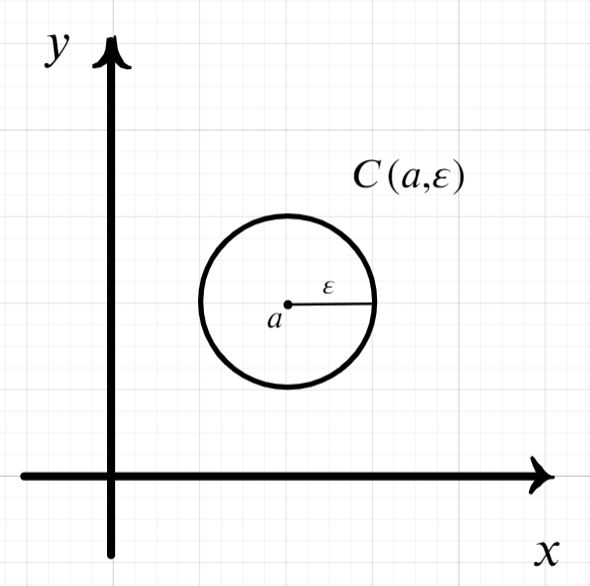
\includegraphics[scale=0.3]{images/009.png}}
\hfill
\parbox[b][4cm][t]{110mm}{Геометрически это множество точек плоскости таких, что $|z-a| = \epsilon$ (расстояние от точки $z$ до точки $a$), то есть это окружность радиуса $\epsilon$ с центром с точке $a$. Обозначается $C(a,\epsilon)$.\\\\Если $|z-a|\leqslant \epsilon$, то это круг с границей радиуса $\epsilon$ с центром с точке $a$. Обозначается $\overline{B}(a,\epsilon)$.\\\\
	Если $|z-a|< \epsilon$, то это круг без границы радиуса $\epsilon$ с центром с точке $a$. Обозначается ${B}(a,\epsilon)$.}\\\\
\begin{center}
	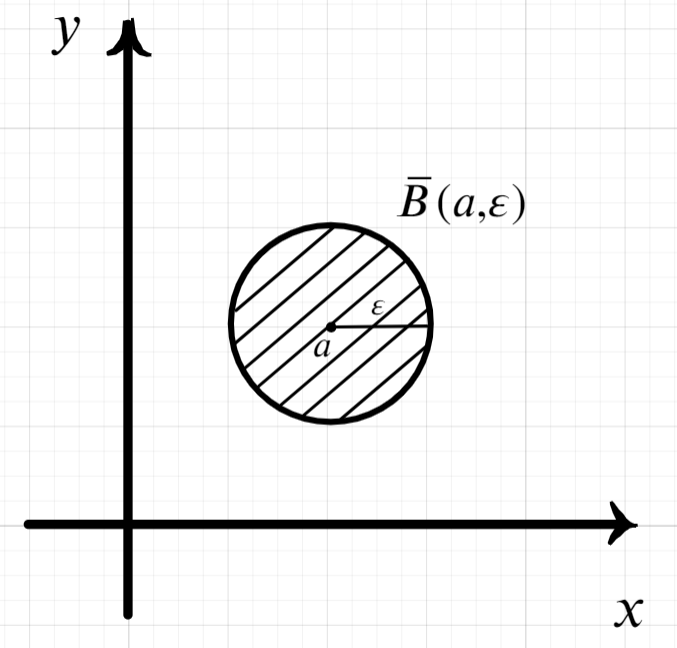
\includegraphics[scale=0.3]{images/010.png}\qquad\qquad\qquad\qquad
	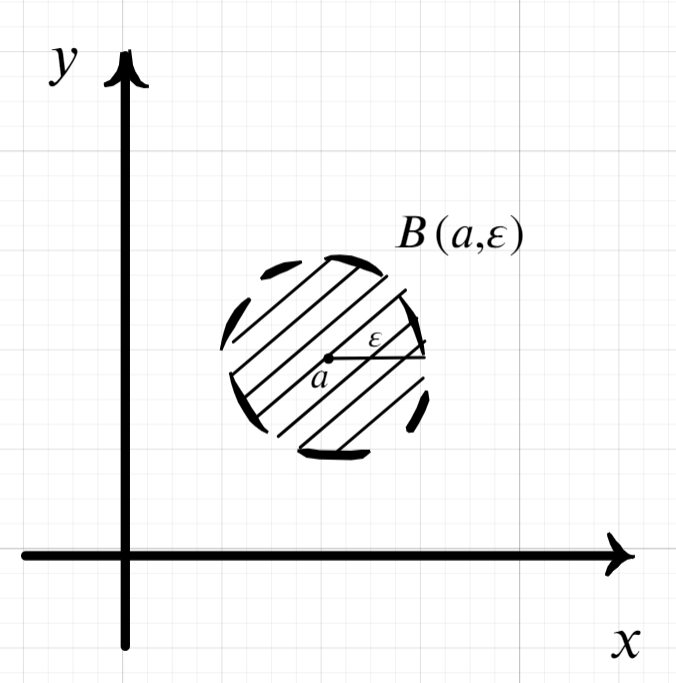
\includegraphics[scale=0.3]{images/011.png}
\end{center}
\noindent
\parbox[b][4.5cm][t]{95mm}{
	$B(a,\epsilon)$ --- $\epsilon$-окрестность точки $a$. $\overline{B}(a,\epsilon)$ --- замкнутая $\epsilon$-окрестность точки $a$.\\\\
	Таким образом, число $a\in \Cm$ --- предел последовательности, если $\limdef$ такое, что все члены последовательности $z_n$ с номерами $\geqslant$ чем $\delta (\epsilon)$ лежат в замкнутой $\epsilon$-окрестности числа $a$.\\\\
}
\hfill
\parbox[b][4.5cm][t]{70mm}{
	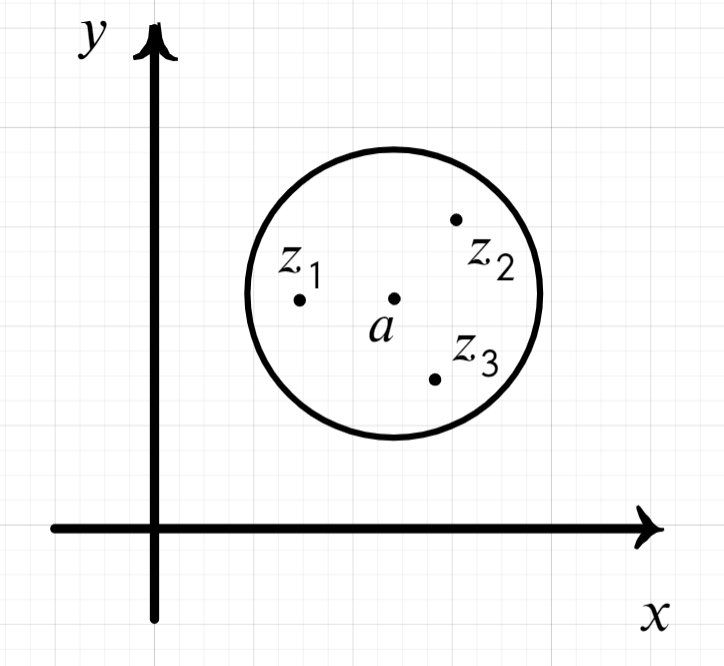
\includegraphics[scale=0.25]{images/012.png}}\\
Говорят, что $(z_n)\underset{n\to\infty}{\longrightarrow} \infty$, если $$\limdef:\forall \geqslant \delta (\epsilon)\Rightarrow |z_n|\geqslant\epsilon,$$
то есть если $\limdef$ такое, что все члены последовательности $z$ лежат вне $\epsilon$-окрестности числа $a$, или $z_n \not \in B(a,\epsilon)$.\\\\
\noindent
\parbox[b][4.5cm][t]{10mm}{
	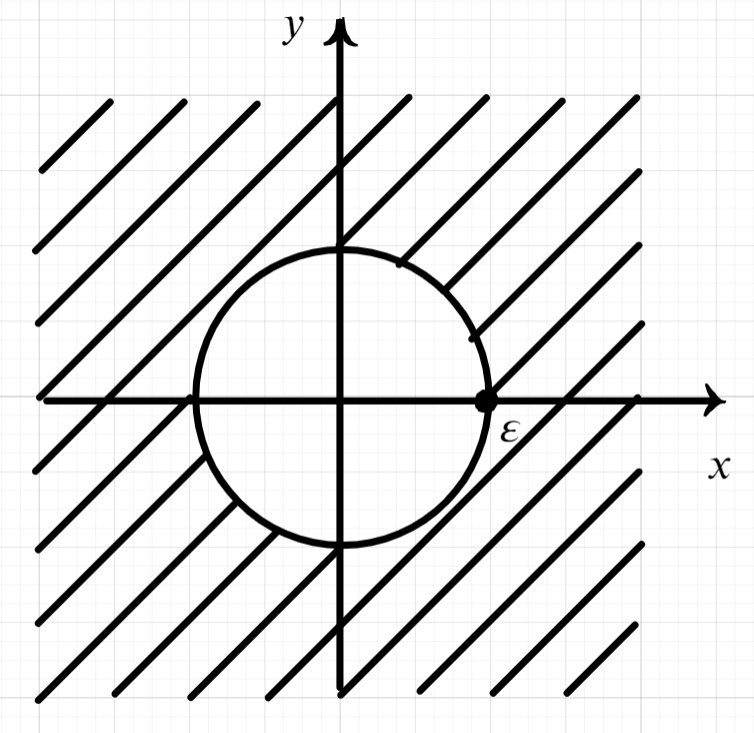
\includegraphics[scale=0.25]{images/014.png}}
\hfill
\parbox[b][4.5cm][t]{110mm}{Дополним множество комплексных чисел $\Cm$ еще одним числом $z = \infty$.\\\\
	$\bullet$ \textit{Множество комплексных чисел, дополненных числом $z = \infty$, называется \textbf{расширенным множествомкомплексных чисел}.}\\\\
	Множество таких $z$, что $|z|>\epsilon$ изображается графически (рис. слева)}\\\\
и называется \textbf{окрестностью бесконечности}.\\\\
$\bullet$ \textit{Комлексная плоскость, дополненная точкой $z = \infty$, называется \textbf{расширенной комплексной плоскостью}.}\\\\
Рассмотрим $(z_n)$, где все члены записываются в алгебраической форме: $z_n = x_n + i\cdot y_n$, $x_n,y_n \in \Rm$.
\begin{theorem}
	$z_n \underset{n\to\infty}{\longrightarrow} a = a_1 + i\cdot a_2 \Longleftrightarrow x_n \underset{n\to\infty}{\longrightarrow} a_1,\ y_n \underset{n\to\infty}{\longrightarrow}a_2$.
\end{theorem}
\begin{Proof}
	$\Rightarrow)$ $z_n \underset{n\to\infty}{\longrightarrow} a$, это значит, что $$\limdef : \forall n \geqslant \delta (\epsilon)\Rightarrow |z_n - a| \leqslant \epsilon.$$
	Так как\\
	\noindent
	\parbox[b][4.5cm][t]{10mm}{
		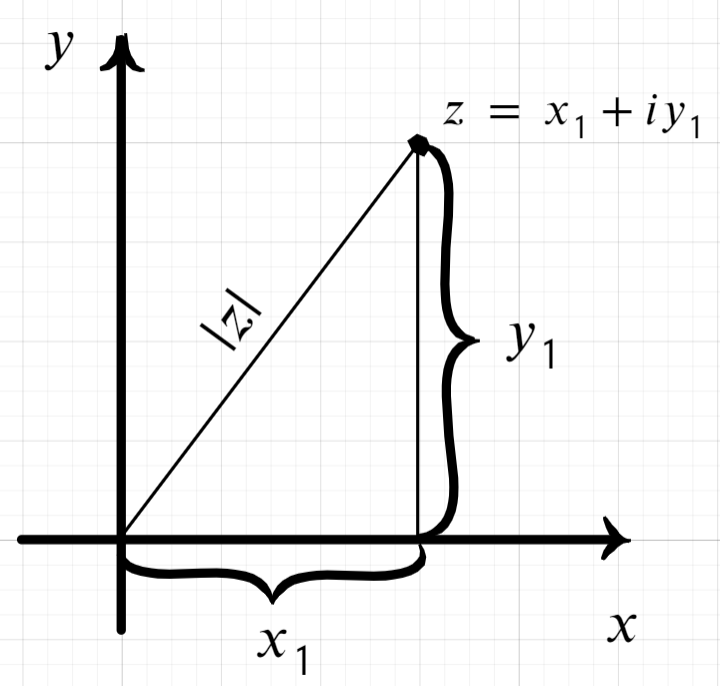
\includegraphics[scale=0.25]{images/015.png}}
	\hfill
	\parbox[b][4cm][t]{100mm}{	то есть $|z| > y$, $|z|>x$, то $$|x_n - a_1|\leqslant |z_n - a|\leqslant \epsilon,$$
		$$|y_n - a_2|\leqslant |z_n - a|\leqslant \epsilon.$$
		Это означает, что $\begin{matrix}
			x_n\underset{n\to\infty}{\longrightarrow}a_1\\
			y_n\underset{n\to\infty}{\longrightarrow}a_2
		\end{matrix}$.
		}\\\\
	$\Leftarrow)$ $\begin{matrix}
		x_n\underset{n\to\infty}{\longrightarrow}a_1\\
		y_n\underset{n\to\infty}{\longrightarrow}a_2
	\end{matrix}$, это значит, что $$\limdef : \forall n \geqslant \delta_1 (\epsilon)\Rightarrow |x_n - a_1| \leqslant \epsilon,$$
$$\limdef : \forall n \geqslant \delta_2 (\epsilon)\Rightarrow |y_n - a_2| \leqslant \epsilon.$$
Тогда $$|z_n - a| = \sqrt{(x_n - a_1)^2 + (y_n-a_2)^2}\leqslant \sqrt{2}\epsilon,\quad \forall n \geqslant \max\{\delta _1(\epsilon), \delta_2(\epsilon)\},$$
а это и есть $z_n \underset{n\to\infty}{\longrightarrow}a$ по $M$-лемме для последовательностей.
\end{Proof}\\\\
\textbf{Замечание.} Если члены последовательности записаны в экспоненциальной форме $z_n = \rho_n e^{i\varphi_n}$, то $z_n \underset{n\to\infty}{\longrightarrow} a = \rho e^{i\varphi_0} \not\Leftrightarrow \rho_n \underset{n\to\infty}{\longrightarrow}\rho$, $\varphi_n \underset{n\to\infty}{\longrightarrow}\varphi_0$, так как $\varphi_n$ определено неоднозначно. Выполняется только $$\rho_n \underset{n\to\infty}{\longrightarrow}\rho,\ \varphi_n \underset{n\to\infty}{\longrightarrow}\varphi_0 \Longrightarrow z_n \underset{n\to\infty}{\longrightarrow} a = \rho e^{i\varphi_0}.$$
Рассмотрим функцию $w = f(z)$, $z\in D\subseteq\Cm$. Любую функцию можно записать как $$w = f(z) = f(x+i\cdot y) = u(x,y) + i\cdot v(x,y),\quad u(x,y)\in \Re(f(z)), v(x,y)\in \Im(f(z)),$$ где $u(x,y)$ и $v(x,y)$ --- вещественные Ф2П.\\\\
Пусть точка $z_0$ --- вутрення точка множества $D$.\\\\
$\bullet$ \textit{Множество $D\backslash\{z_0\}$ называется \textbf{проколотой окрестностью} точки $z_0$.}\\\\
$\bullet$ \textit{Число $A\in \Cm$ называется \textbf{пределом функции} $f(z)$ при $z\to z_0$, если} $$\limdef,\ \forall z : 0 < |z-z_0|\leqslant\delta(\epsilon)\Rightarrow |f(z) - A|\leqslant\epsilon.$$
То есть $\limdef$ такое, что для всех $z$ из проколотой $\delta$-окрестности точки $z_0$ функция $f(z)$ принимает значения в $\epsilon$-окрестности числа $A$. Пишут $\lim\limits_{z\to z_0} f(z) = A$, или $f(z)\underset{z\to z_0}{\longrightarrow}A.$
$$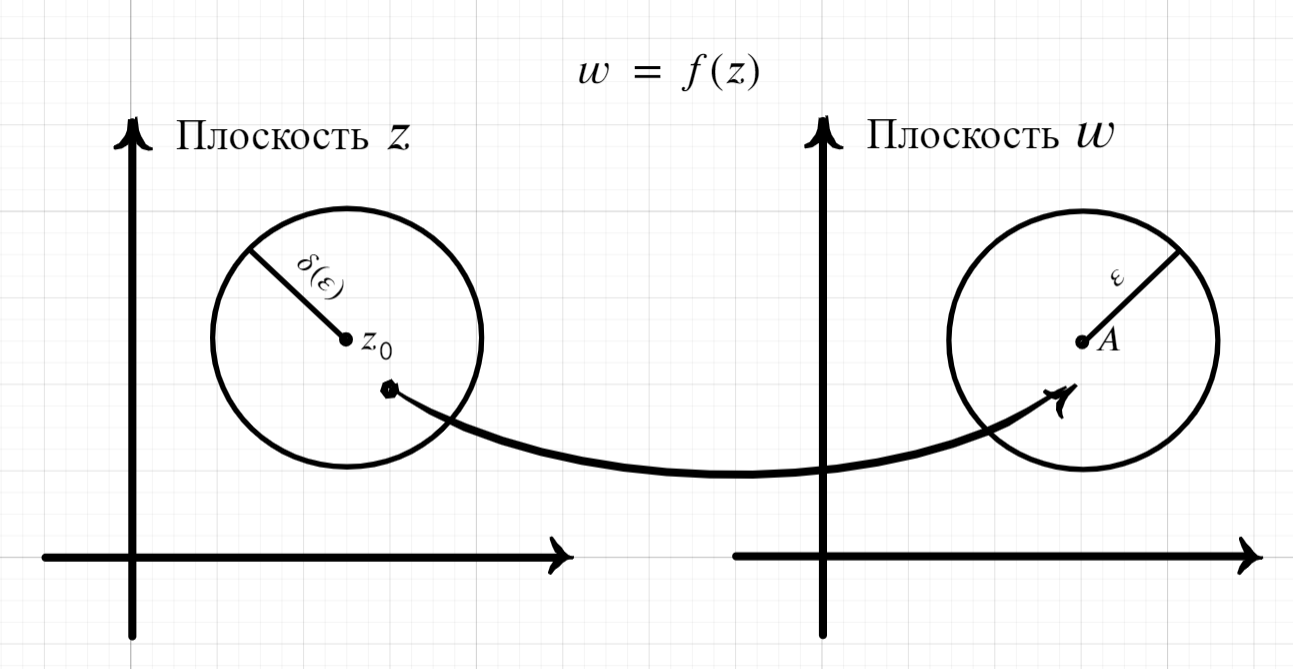
\includegraphics[scale=0.4]{images/016.png}$$
Когда мы говорим о пределе функции, мы рассматриваем лишь однозначные функции.\\\\
Число $A$ может быть и $\infty$. Пусть $A = \infty$, тогда $f\underset{z\to \infty}{\longrightarrow}\infty$, если $$\limdef\ \forall z : |z|\geqslant \delta (\epsilon) \Rightarrow |f(z)|\geqslant \epsilon.$$
\textbf{Теорема.}
	$f(z)\underset{z\to z_0}{\longrightarrow}A = B + i\cdot D \Longleftrightarrow u(x,y)\underset{\underset{y\to y_0}{x\to x_0}
	}{\longrightarrow}B$, $v(x,y)\underset{\underset{y\to y_0}{x\to x_0}}{\longrightarrow}D$.\\\\
Пусть $z_0$ --- предельная точка множества $D$, а $w = f(z)$.\\\\
$\bullet$ \textit{Число $A$ --- \textbf{предел функции} $f(z)$ при $z \to z_0$ \textbf{вдоль множества} $D$, если} $$\limdef,\ \forall z \in D\backslash\{z_0\} : 0 < |z-z_0|\leqslant\delta(\epsilon)\Rightarrow |f(z) - A|\leqslant\epsilon.$$
Тогда пишут $\lim\limits_{\underset{z\in D}{z\to z_0}}f(z) = A$.\\\\
\textit{\textbf{Свойства предела функции:}}\begin{enumerate}
	\item \textbf{\textit{Единственность.}} \textit{Предел функции, если он существует, определен однозначно.}
	\item \textit{Если $f(z)\underset{z\to z_0}{\longrightarrow} A\in \Cm$, то функция ограничена в некоторой проколотой окрестности точки $z_0$.}
	\item \textit{Если $\lim\limits_{z\to z_0}f(z) = A$, $\lim\limits_{z\to z_0}f(z) = B$, $A, B\in\Cm$, то}\begin{enumerate}
		\item $\lim\limits_{z\to z_0}\Big(f(z) + g(z)\Big) = \lim\limits_{z\to z_0}f(z) + \lim\limits_{z\to z_0}g(z);$
		\item $\lim\limits_{z\to z_0}\Big(f(z) \cdot g(z)\Big) = \lim\limits_{z\to z_0}f(z) \cdot  \lim\limits_{z\to z_0}g(z);$
		\item $\lim\limits_{z\to z_0}\dfrac{f(z)}{g(z)} = \dfrac{\lim\limits_{z\to z_0}f(z)}{\lim\limits_{z\to z_0}g(z)},$ \textit{если} $\lim\limits_{z\to z_0}g(z)\ne 0$.
	\end{enumerate}
\end{enumerate}
Пишем $f(z)\underset{z\to z_0}{\sim}g(z)$, если $\lim\limits_{z\to z_0}\dfrac{f(z)}{g(z)} = 1.$\\\\
Пишем $f(z)\underset{z\to z_0}{=}o(g(z))$, если $\lim\limits_{z\to z_0}\dfrac{f(z)}{g(z)} = 0.$\\\\
При вычислении пределов функцию можно также заменить на эквивалентную ей.\\\\
Рассмотрим функцию $w = f(z)$ определенную в окрестности точки $z_0\in D$ (внутренняя точка). \\\\
$\bullet$ \textit{Функцию $f(z)$ называют \textbf{непрерывной в точке} $z_0$, если} $$\lim\limits_{z\to z_0} f(z) = f(z_0).$$
$\bullet$ \textit{Если точка $z_0 \in D$ является предельной, то при $\lim\limits_{z\to z_0} f(z) = f(z_0)$ функция $f$ \textbf{непрерывна в точке $z_0$ вдоль множества $D$}.}\\\\
Любую функцию можно записать в виде $$w = f(z) = u(x,y) + i\cdot v(x,y).$$
Функция $f(z)$ непрерывна в точке $z_0$ $\Longleftrightarrow$ $u(x,y)$, $v(x,y)$ непрерывны в точке $(x_0,y_0)$, где $x_0 + i\cdot y_0 = z_0$ (следует из определения).\\\\
\textbf{\textit{Свойства непрерывных функций:}}\begin{enumerate}
	\item \begin{enumerate}
		\item $f(z) + g(z)$ \textit{непрерывна};
		\item $f(z)\cdot g(z)$ \textit{непрерывна};
		\item $\dfrac{f(z)}{g(z)}$ \textit{непрерывна} ($g(z)\ne 0$),
	\end{enumerate}
	\textit{если функции $f(z)$ и $g(z)$ непрерывны в точке $z$.}
	\item \textit{Если $w = F(z)$, $z = \varphi(\zeta)$, причем $\varphi(\zeta)$ непрерывна в точке $\zeta_0$, а $F(z)$ непрерывна в точке $z_0 = \varphi(\zeta_0)$, то $F(\varphi(\zeta))$ непрерывна в точке $\zeta_0$ (композиция непрерывных функций является функцией непрерывной).}
	\item \textbf{(Теорема Кантора.)}\\
	\textit{Непрерывная на компакте $D$ функция $w = f(z)$ равномерно непрерывна, то есть }$$\limdef,\ \forall z',z'' \in D : |z' - z''|\leq\delta(\epsilon)\Rightarrow |f(z') - f(z'')|\leq \epsilon.$$
\end{enumerate}
\section{Дифференцирование комплексных функций.}
Пусть $w = f(z)$ определена в окрестности точки $z_0$. Построим приращение $$\Delta f = f(z_0 + \Delta z) - f(z_0).$$
$\bullet$ \textit{\textbf{Производной комплексной функции} называется предел (если он конечен) }$$\lim\limits_{\Delta z\to 0}\dfrac{\Delta f}{\Delta z} = f'(z_0) = f'(z)|_{z=z_0}.$$
Тогда будем говорить, что комплексная функция имеет конечную производную.\\\\
$\bullet$ \textit{Функцию $w = f(z)$ называют \textbf{дифференцируемой} в точке $z_0$, если} $\exists A \in \Cm :$ $$\Delta f = A\cdot \Delta z + o(\Delta z).$$
\textbf{Первый критерий дифференцируемости функции.} \textit{Фукнция $f(z)$ дифференцируема в точке $z_0$ $\Longleftrightarrow$ она имеет конечную производную в этой точке $f'(z_0)$.}\\\\
\begin{Proof}
	$\Rightarrow)$ Поскольку $\Delta f = A\cdot \Delta z  + o(\Delta z)$, то
	$$\dfrac{\Delta f}{\Delta z} = A + \dfrac{o(\Delta z)}{\Delta z}.$$
	Переходим к пределу при $\Delta z \to 0$:
	$$\lim\limits_{\Delta z \to 0}\dfrac{\Delta f}{\Delta z} = A\Rightarrow f'(z_0) = A.$$
	$\Leftarrow)$ $\lim\limits_{\Delta z\to 0}\dfrac{\Delta f}{\Delta z} = f'(z_0)$. Отсюда $$\lim\limits_{\Delta z\to 0}\Big(\dfrac{\Delta f}{\Delta z} - f'(z_0)\Big) = 0;$$
	$$\dfrac{\Delta f}{\Delta z} - f'(z_0) = o(1);$$
	$$\Delta f = f'(z_0)\cdot \Delta z + \Delta z \cdot o(1) = f'(z_0)\cdot \Delta z +o(\Delta z ),$$ 
	то есть функция дифференцируема в точке $z_0$.
\end{Proof}\\\\
\textbf{Замечание.} \textit{$o(\Delta z) = o(|\Delta z|)$, докажем это.} $$o(\Delta z) = \alpha (\Delta z) \Rightarrow \lim\limits_{\Delta z \to 0} \dfrac{\alpha (\Delta z)}{\Delta z} = 0;\eqno (*)$$
$$o(|\Delta z|) = \alpha (|\Delta z|) \Rightarrow \lim\limits_{\Delta z \to 0} \dfrac{\alpha (|\Delta z|)}{|\Delta z|} = 0.\eqno (**)$$
\textit{Тогда} $$\lim\limits_{\Delta z \to 0}\dfrac{\alpha (\Delta z)}{\Delta z} = \lim\limits_{\Delta z\to 0}\dfrac{\alpha (\Delta z)}{\Delta z}\cdot \dfrac{\Delta z}{|\Delta z|} = 0.$$
\textit{Соответственно, если выполняется $(*)$, то выполняется и $(**)$, и наоборот. Из этого следует, что дифференциал можно также записать в виде} $$\Delta f = A\cdot \Delta z + o(|\Delta z|).$$
\textbf{Второй критерий дифференцируемости функции.} \textit{Функция $f(z) = u(x,y) + i\cdot v(x,y)$ дифференцируема в точке $z_0 = x_0 + i\cdot y_0$ $\Longleftrightarrow$ \begin{enumerate}
		\item функции $u(x,y)$, $v(x,y)$ дифференцируемы в точке $(x_0,y_0)$;
		\item выполняются условия Коши-Римана: в точке $(x_0, y_0)$
		$$\dfrac{\d u}{\d x} = \dfrac{\d v}{\d y},\quad \dfrac{\d u}{\d y} = -\dfrac{\d v}{\d x}.$$
\end{enumerate}
Причем $$f'(z)|_{z=z_0} = \dfrac{\d u}{\d x}\Big |_{(x_0,y_0)} + i\cdot \dfrac{\d v}{\d x}\Big |_{(x_0,y_0)}.$$}
\begin{Proof}
	$\Rightarrow)$ $\Delta f = A\cdot \Delta z + o(\Delta z)$, где $$A = B_1 +i\cdot B_2,$$ $$\Delta f = \Delta u + i\cdot \Delta v,$$ $$\Delta z = \Delta x + i\cdot \Delta y,$$ $$o(\Delta z) = \epsilon_1 + i\cdot \epsilon_2.$$ Тогда $$\Delta f = \Delta u + i\cdot \Delta v = (B_1 + i\cdot B_2)(\Delta x + i\cdot \Delta y) + \epsilon_1 + i\cdot \epsilon_2.$$
	Отсюда $$\Delta u = B_1\Delta x - B_2\Delta y + \epsilon_1,\quad \Delta v = B_2\Delta x + B_1\Delta y + \epsilon_2;$$
	причем $|\epsilon_1|\leqslant |o(\Delta z)|$, $|\epsilon_1| = o(|\Delta z|) = o(\sqrt{(\Delta x)^2 + (\Delta y)^2})$. Аналогично $|\epsilon_2| =  o(\sqrt{(\Delta x)^2 + (\Delta y)^2})$. Подставим и получим $$\Delta u = B_1\Delta x - B_2\Delta y + o(\sqrt{(\Delta x)^2 + (\Delta y)^2}),\quad \Delta v = B_2\Delta x + B_1\Delta y + o(\sqrt{(\Delta x)^2 + (\Delta y)^2}).$$
	Вспомним, что\\\\
	\textit{Функция $f(x,y)$ называется дифференцируемой в точке $(x_0,y_0)$, если $\exists A,D\in \Rm : $ $$\Delta f = A\cdot \Delta x + D\cdot \Delta y + o(\sqrt{(\Delta x)^2 + (\Delta y)^2}),$$
	причем $A = f'_x$, $D = f'_y$.}\\\\
	Тогда $u(x,y)$ является дифференцируемой в точке $(x_0,y_0)$ и $$\dfrac{\d u}{\d x} = B_1,\quad \dfrac{\d u}{\d y} = -B_2.$$
	Но $v(x,y)$ также является дифференцируемой в точке $(x_0,y_0)$ и$$\dfrac{\d v}{\d x} = B_2,\quad \dfrac{\d v}{\d y} = B_1.$$
	Следовательно, $$\dfrac{\d u}{\d x} = \dfrac{\d v}{\d y},\quad \dfrac{\d u}{\d y} = -\dfrac{\d v}{\d x}.$$
	$\Leftarrow)$ Для доказательства все рассуждения проведем в обратном порядке. Так как $u(x,y)$ и $v(x,y)$ дифференцируемы в точке $(x_0,y_0)$, то в этой точке $$\Delta u = \dfrac{\d u}{\d x}\Delta x + \dfrac{\d u}{\d y}\Delta y + o_1(\sqrt{(\Delta x)^2 + (\Delta y)^2}),$$
	$$\Delta v = \dfrac{\d v}{\d x}\Delta x + \dfrac{\d v}{\d y}\Delta y + o_2(\sqrt{(\Delta x)^2 + (\Delta y)^2}).$$
	Тогда\begin{multline*}
		\Delta f = \Big(\dfrac{\d u}{\d x}\Delta x+ i\cdot \dfrac{\d v}{\d x}\Delta x\Big) + \Big(-\dfrac{\d v}{\d x}\Delta y + i\cdot \dfrac{\d u}{\d x}\Delta y\Big) + \underbrace{o_1(\sqrt{(\Delta x)^2 + (\Delta y)^2}) + o_2(\sqrt{(\Delta x)^2 + (\Delta y)^2})}_{o(\Delta z)}=\\=\dfrac{\d u}{\d x}\underbrace{(\Delta x + i\cdot \Delta y)}_{\Delta z} + i\cdot \dfrac{\d v}{\d x}\underbrace{(\Delta x + i\cdot \Delta y)}_{\Delta z} + o(\Delta z) = \Big(\dfrac{\d u}{\d x} + i\cdot \dfrac{\d v}{\d x}\Big)\cdot \Delta z + o(\Delta z).
	\end{multline*}
Следовательно, $f(z)$ дифференцируема в точке $z_0$, а $$f'(z_0) = \dfrac{\d u}{\d x}\Big |_{(x_0,y_0)} + i\cdot \dfrac{\d v}{\d x}\Big |_{(x_0,y_0)}.$$
\end{Proof}
\end{document}
